\documentclass[a4paper,11pt]{article}
\usepackage[utf8]{inputenc}
\usepackage[margin=2cm]{geometry}
\usepackage{enumitem}
\usepackage{hyperref}
\usepackage{xcolor}
\usepackage{graphicx}
\graphicspath{{img/}}
\usepackage{float}
\usepackage{lipsum}
\usepackage{multicol}
\usepackage{tabto}
\usepackage[most]{tcolorbox}
%\usepackage{showframe} % Carga el paquete para mostrar los márgenes

\usepackage{parskip}
\usepackage{ragged2e}

\usepackage{progressbar} % Carga el paquete "progressbar" para crear barras de progreso.
\usepackage{xcolor} % Carga el paquete "xcolor" para manejar colores.

\newcommand{\progressline}[2]{ % Define un nuevo comando llamado \progressline que toma dos argumentos.
	\progressbar[width=4cm, linecolor=blue, filledcolor=darkblue!50]{#1} % Crea una barra de progreso con el ancho del texto, color de línea azul y color de relleno azul claro.
	\hspace{5pt} % Agrega un espacio horizontal de 5 puntos.
	#2 % Muestra el segundo argumento, que es la indicación de progreso.
}

\usepackage[spanish]{babel}

%\usepackage{helvet} % Cargar el paquete helvet para la fuente sans serif
\renewcommand{\familydefault}{\sfdefault} % Cambiar la familia de fuente por defecto a sans serif
%\usepackage{fontspec}

\usepackage{fontawesome}  %Paquete de iconos


\definecolor{darkblue}{RGB}{0,0,128}
\definecolor{lightblue}{RGB}{173,216,230}

\pagestyle{empty}

\begin{document}	
		%\setmainfont{Times New Roman}	
		\begin{tcolorbox}[
			enhanced,
			boxrule=2pt,
			colframe=darkblue,
			colback=darkblue,
			width=\linewidth,
			sharp corners,
			halign=center, % Centrar el contenido horizontalmente
			valign=center, % Centrar el contenido verticalmente
			]
			\color{white} \Large{\textbf{CURRICULUM VITAE}}
		\end{tcolorbox}
	
	
	\begin{multicols}{2}[\columnsep=0.4cm] % Espacio entre columnas
			
		\begin{center}
			\begin{minipage}{0.4\textwidth}
				\centering
				\begin{center}
					\fbox{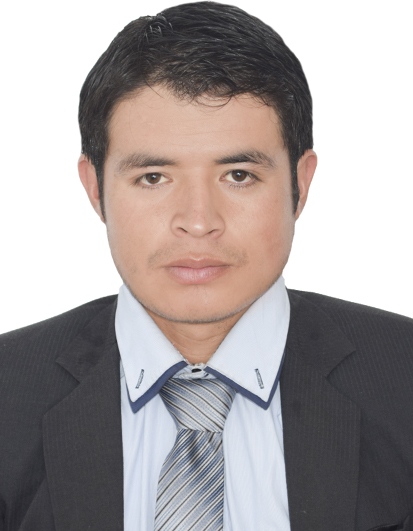
\includegraphics[width=3cm]{0.0.jpg}}
				\end{center}
				%\textcolor{darkblue}{\rule{\textwidth}{1pt}} 
				\textcolor{darkblue}{\Large \textbf{Juan Benito}\\ \textbf{Quintana Arone}} \\
				\textcolor{darkblue}{\rule{\linewidth}{2pt}} % Línea horizontal azul del ancho del texto con grosor de 1.5pt
				\vspace{0.3mm}
				\textcolor{darkblue}{\large \textbf{Egresado}}
				\vspace{0.3mm}
				\textcolor{darkblue}{\rule{\linewidth}{2pt}} % Línea horizontal azul del ancho del texto con grosor de 1.5pt
			\end{minipage}
			
		\end{center}
		
% Acerca de mi %%%%%%%%%%%%%%%%%%%%%%%%%%%%%%%%%%%%%%%%%%%%%%%%%%%%%%%%%%%%%%%%%%%%%%%%%%%%%%

			\begin{center}
				\begin{minipage}{0.4\textwidth}
					
					\begin{tcolorbox}[
						enhanced,
						boxrule=2pt,
						colframe=darkblue,
						colback=darkblue!10,
						width=\linewidth,
						sharp corners,
						halign=center,  %Tener en cuenta para imprimir cambiar a flush
						valign=center,
						title=\begin{center}
							\section*{Acerca de mí}
						\end{center}, % Título de la caja
						]				
						Egresado de Ingeniería Civil, me considero una persona creativa y responsable con iniciativa y puntualidad, asumo con agrado los retos y metas que su organización me pudiera plantear, con un buen manejo de relaciones interpersonales facilidad para trabajar en equipo y en condiciones de presión ; acostumbrado a actuar en entornos con plazos determinados, haciendo hincapié en trabajar dentro de los requisitos presupuestarios.\\
						Habilidades de comunicación escrita y verbal bien desarrolladas.
						Altamente capacitado en las relaciones y negociaciones con clientes y proveedores.	
					\end{tcolorbox}
					
				\end{minipage}
			\end{center}

\vspace{5mm}	
% Contacto %%%%%%%%%%%%%%%%%%%%%%%%%%%%%%%%%%%%%%%%%%%%%%%%%%%%%%%%%%%%%%%%%%%%%%%%%%%%%
	
		\begin{center}
			\begin{minipage}{0.41\textwidth}
				
				\begin{tcolorbox}[
					enhanced,
					boxrule=2pt,
					colframe=darkblue,
					colback=darkblue!10,
					width=\linewidth,
					sharp corners,
					halign=center,  %Tener en cuenta para imprimir cambiar a flush
					valign=center,
					title=\begin{center}
						\section*{Contacto}
					\end{center}, % Título de la caja
					]				
					\begin{tabbing}
						\hspace{1.8cm} \= \hspace{4cm} \= \kill % Establecer las tabulaciones
						\textbf{Dirección:} \> Av. Diamont \\
						\> -Tamburco-Abancay \> \\
						\textbf{\faPhoneSquare Teléfono:}  \> 988757518 \> \\
						\textbf{\faEnvelope Email:} \> juanbenito01qa@gmail.com \> \\
					\end{tabbing}	
				\end{tcolorbox}
				
			\end{minipage}
		\end{center}
\vspace{5mm}
% IDIOMAS %%%%%%%%%%%%%%%%%%%%%%%%%%%%%%%%%%%%%%%%%%%%%%%%%%%%%%%%%%%%%%%%%%%%%%%%%%%%%%
		\begin{center}
			\begin{minipage}{0.4\textwidth}
				
				\begin{tcolorbox}[
					enhanced,
					boxrule=2pt,
					colframe=darkblue,
					colback=darkblue!10,
					width=\linewidth,
					sharp corners,
					halign=center,  %Tener en cuenta para imprimir cambiar a flush
					valign=center,
					title=\begin{center}
							\section*{Idiomas}
						  \end{center}, % Título de la caja
					]				
					\begin{tabbing}
						\hspace{1.6cm} \= \hspace{4cm} \= \kill % Establecer las tabulaciones
						Español: \> \progressline{0.9} \\
						Quechua: \> \progressline{0.9} \> \\
						Inglés: \> \progressline{0.4} \> \\
					\end{tabbing}	
				\end{tcolorbox}
				
			\end{minipage}
		\end{center}

%Formación %%%%%%%%%%%%%%%%%%%%%%%%%%%%%%%%%%%%%%%%%%%%%%%%%%%%%%%%%%%%%%%%%%%%%%%%%%%%%	
	%\vspace{0.5cm}
	
		\section*{\textcolor{darkblue}{Formación}}
		\textbf{Universidad Nacional Micaela Bastidas de Apurímac}\\
		\textit{Escuela Académico Profesional de Ingeniería Civil}
		(2018-2023)
		%\vspace{0.4cm}
		
		\noindent \textbf{Universidad Nacional San Antonio Abad del Cusco}\\
		\textit{Facultad  de Ciencias Biológicas la carrera de Biología}
		(2010-2013)
		

% Formación %%%%%%%%%%%%%%%%%%%%%%%%%%%%%%%%%%%%%%%%%%%%%%%%%%%%%%%%%%%%%%%%%%%%%%%%%%%%%%		
		\section*{\textcolor{darkblue}{Experiencia Laboral}}
		
		\textbf{Municipalidad Distrital de Tamburco} \\
		\textit{Oficina de obras} \\
		\\ Obra: “Mejoramiento y ampliación de los servicios de agua potable y sistemas de saneamiento básico rural en 26 localidades del distrito de Mariscal Gamarra, provincia de Grau - región Apurímac”\\
		\textit{4 de abril a 28 de noviembre  de 2018}\\
		
		\textbf{Consorcio Andino-Constructora Sondor} \\

		 Obra: “Mejoramiento y ampliación de los servicios de agua potable y sistemas de saneamiento básico rural en 26 localidades del distrito de Mariscal Gamarra, provincia de Grau - región Apurímac”\\
		\textit{4 de abril a 28 de noviembre  de 2018}\\
		
% Habilidades tecnicas %%%%%%%%%%%%%%%%%%%%%%%%%%%%%%%%%%%%%%%%%%%%%%%%%%%%%%%%%%%%%%%%%%		
		\section*{\textcolor{darkblue}{Habilidades Técnicas}}
		\noindent \textbf{Creación y edición de documentos científicos y técnicos utilizando \LaTeX.}
		
		\begin{tabbing}
			\hspace{3cm} \= \hspace{5cm} \= \kill % Establecer las tabulaciones
			\LaTeX: \> \progressline{0.9} \\
			Beamer: \> \progressline{0.9} \> \\
		\end{tabbing}

\newpage
%MathCAD prime v9
	\noindent \textbf{Creación y edición de documentos técnicos utilizando MathCAD Prime v9.}
	
	\begin{tabbing}
		\hspace{3cm} \= \hspace{5cm} \= \kill % Establecer las tabulaciones
		MathCAD Prime: \> \progressline{0.7} \> \\
	\end{tabbing}

		\noindent \textbf{Paquete de programas de Microsoft}
		
		\begin{tabbing}
			\hspace{3cm} \= \hspace{5cm} \= \kill % Establecer las tabulaciones
			Word: \> \progressline{0.9} \\
			Excel: \> \progressline{0.9} \> \\
			Power Point: \> \progressline{0.9} \> \\
		\end{tabbing}
		
		\noindent \textbf{Paquete de programas de Autodesk 2024}
		\begin{tabbing}
			\hspace{3cm} \= \hspace{5cm} \= \kill % Establecer las tabulaciones
			AutoCAD: \> \progressline{0.9} \\
			Civil 3D: \> \progressline{0.9} \> \\
			Revit: \> \progressline{0.5} \> \\
		\end{tabbing}
		
		\noindent \textbf{Software costos y presupuestos}
		\begin{tabbing}
			\hspace{3cm} \= \hspace{5cm} \= \kill % Establecer las tabulaciones
			Power Cost: \> \progressline{0.8} \\
		\end{tabbing}

		\noindent \textbf{Paquete de programas Adobe}
		\begin{justify}
			\begin{tabbing}
				\hspace{3cm} \= \hspace{5cm} \= \kill % Establecer las tabulaciones
				Illustrator: \> \progressline{0.8} \\
			\end{tabbing}
		\end{justify}
		
		\noindent \textbf{Control y seguimiento de proyectos con Oracle}
		\begin{justify}
			\begin{tabbing}
				\hspace{3cm} \= \hspace{5cm} \= \kill % Establecer las tabulaciones
			Primavera P6: \> \progressline{0.8} \\
			\end{tabbing}
		\end{justify}
		
		\noindent \textbf{Análisis de datos geoespaciales}
		\begin{justify}
			\begin{tabbing}
				\hspace{3cm} \= \hspace{5cm} \= \kill % Establecer las tabulaciones
				QGis: \> \progressline{0.8} \\
			\end{tabbing}
		\end{justify}
		
%\section*{\textcolor{darkblue}{Referencias}}	
	\end{multicols}
	
\end{document}
